\subsection{Identifying SBOM Tool Metrics}
% TODO: way too small, will fix later
\begin{figure}[h!]
	\centering
	\begin{subfigure}[b]{0.4\linewidth}
		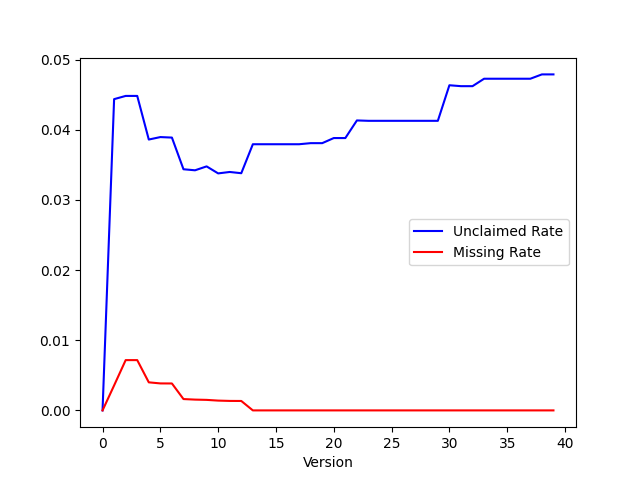
\includegraphics[width=\linewidth]{graph/fig1a.png}
		\caption{Unclaimed \& Missing Rate}
	\end{subfigure}
	\begin{subfigure}[b]{0.4\linewidth}
		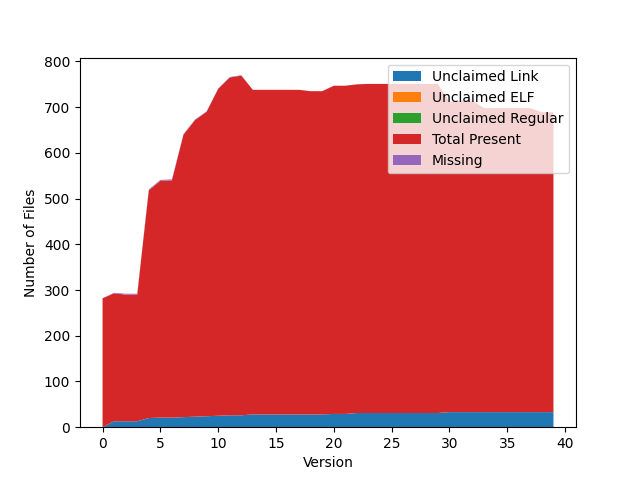
\includegraphics[width=\linewidth]{graph/fig1b.png}
		\caption{Status of All Files}
	\end{subfigure}
	\caption{DiffBOM Results on Openwrt}
	\label{fig:openwrt}
\end{figure}
% Ver mapping table 
\begin{table}[h!]
	\centering
	\begin{tabular}{|c|c|}
		\hline
		Figure Version & OpenWrt Version \\
		\hline
		0 & 0.9 \\
		1 - 3 & 7.06 - 7.09 \\
		4 - 6 & 8.09 - 8.09.2 \\
		7 - 8 & 10.03 - 10.03.1 \\
		9 & 12.09 \\
		10 & 14.07 \\
		11 - 12 & 15.05 - 15.05.1 \\
		13 - 19 & 17.01.0 - 17.01.6 \\
		20 - 29 & 18.06.0 - 18.06.9 \\
		30 - 39 & 19.07.0 - 19.07.9 \\
		\hline
	\end{tabular}
	\caption{Mapping of Version Number in Figure n to OpenWrt Version Number}
	\label{table:openwrt}
\end{table}
We manually collected 40 versions of OpenWrt firmware ranging from version 0.9 to version 19.07.7, available on the OpenWrt Stable Release repository \cite{OpenWrt_Vers}. No SPDX SBOMs are available, and package managers used are ipkg in versions up to ?? and opkg in later versions. Then we run DiffBOM on them to acquire the metrics. The metrics are plotted on Figure n, with the Unclaimed Rate calculated as
\[Unclaimed Rate = \frac{Number of Unclaimed Files}{Total Present Files}\]
and the Missing Rate calculated as
\[Missing Rate = \frac{Number of Missing Files}{Number of Tracked Files + Number of Missing Files}.\]
We also plotted a stacked plot to illustrate the composition of unclaimed files in terms of file types.
The corresponding OpenWrt version numbers are illustrated in Table n. \par
As seen in \ref{fig:openwrt}, the missing rate starts low, showing a little spike across several early versions, then eventually decreases and stays at zero. This signals an improving and then constantly good practice in preserving files installed by package managers. \par
The missing rate, on the other hand, shows constant fluctuation across versions. The first version is a perfect version showing zero unclaimed and missing files. Then the next versions see a great increase in unclaimed rate to almost 5\%. Then until version 15.05.1, a decrease is observed, followed by a constant increase after the version. The increase or decrease roughly follows a spike-stagnate trend, with each significant increase or decrease at roughly the major version number changes, followed by a period of no significant change in between, peaking at below 5\%. This observation aligns with our expectation that most changes occur at major version number bumps. \par
Overall no unclaimed ELF or regular files are present on any versions, all unclaimed files are symbolic links. Upon manual inspection, however, we discover that across all versions, all files under /etc/rc\.d, which are all symbolic links to other scripts, as well as occasional links under /usr/bin, are not tracked. \par
Combined, this signals good practice in managing software packages, and SBOMs from package managers mostly accurately reflects OpenWrt file system status. However, the fact that links to scripts and binaries, which reside in important locations on file system, are constantly unclaimed is alarming.\par
\subsection{Providing Better Guidance for SBOM Tooling}


